\begin{frame}
\frametitle{Suréchantillonnage}

\begin{block}{Objectif}
Diminuer le \emph{crénelage} des images.
\end{block}

\begin{block}{Principe du suréchantillonnage x 8}
\begin{itemize}
\item \pause Envoyer 8 rayons supplémentaires autour du pixel considéré, soit 9 pixels en tout.
\item \pause Faire la moyenne des couleurs obtenues.
\end{itemize}
\end{block}
\end{frame}

\begin{frame}

\frametitle{Résultats obtenus}

\only<1>{
\begin{multicols}{2}
\begin{figure}
\begin{center}
	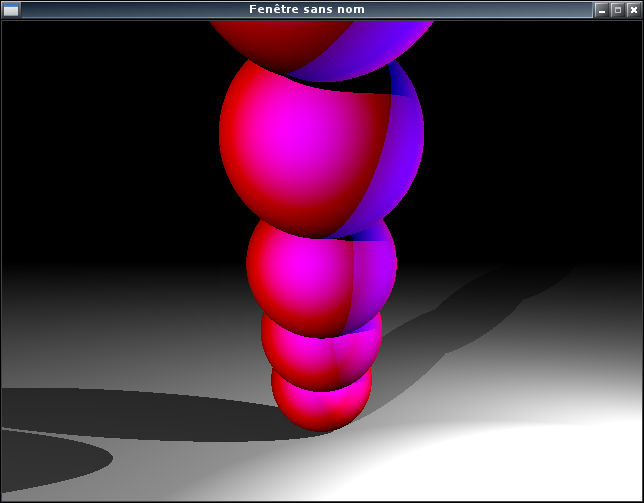
\includegraphics[scale=0.3]{NOver.png}
\end{center}
\caption{Figure crénelée.}
\end{figure}

\begin{figure}
\begin{center}
	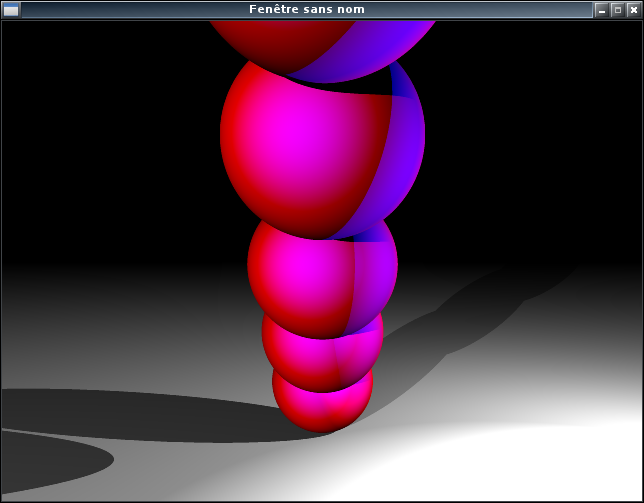
\includegraphics[scale=0.3]{Over.png}
\end{center}
\caption{Avec anti-crénelage par suréchantillonnage x 8.}
\end{figure}

\end{multicols}

}
\only<2>{

\begin{block}{Crenelée}
\begin{center}
	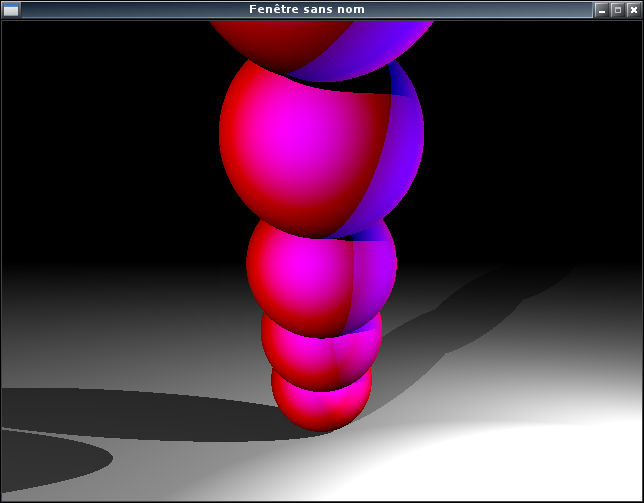
\includegraphics[scale=0.5]{NOver.png}
\end{center}
\end{block}
}

\only<3>
{
\begin{block}{Moins crénelée}
\begin{center}
	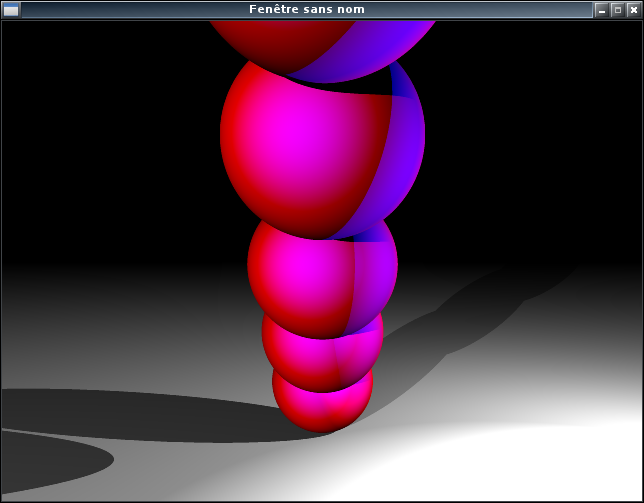
\includegraphics[scale=0.5]{Over.png}
\end{center}
\end{block}
}

\end{frame}

\begin{frame}
\frametitle{Limitations et autres algorithmes}

\begin{alertblock}{Lent}
\emph{Neuf} fois plus de calculs dans le cas du suréchantillonnage x 8.
\end{alertblock}

\only<2>
{
	\begin{block}{Détection de contours}
	\begin{itemize}
	\item L'algorithme détecte les contours dans l'image et par exemple applique un flou à ceux-ci.
	\item C'est plus rapide.
	\item Ca peut échouer sur des images très complexes, avec des contours pas très définis.
	\end{itemize}
	\end{block}
}

\only<3>
{
	\begin{block}{Traitement du signal}
	\begin{itemize}
	\item Créneaux = hautes fréquences
	\item Effectuer une transformée de Fourier de l'image.
	\item Filtrer les hautes fréquences.
	\item Effectuer une transformée inverse de Fourier du spectre obtenu précédemment.
	\end{itemize}
	\end{block}
}

\end{frame}

